\documentclass[12pt, a4paper]{article}

\usepackage{graphicx}
\usepackage{float}
\usepackage{hyperref}
\usepackage{siunitx}
\usepackage{gensymb}

\begin{document}
	\pagenumbering{gobble}
		\begin{titlepage}
			\centering
			{\LARGE Electronics Practical 4 \par}
			\vspace*{1.5cm}
			{\large Q. Kruger, 216008466 \par}
			{\large R. de Bruyn, 216054484 \par}
			{\large W. B. Richardson, 201578882 \par}
			\vspace*{1.2cm}
			{\large \today}
			\vspace*{\fill}
			% 
\includegraphics[width=\textwidth]{img/UJ.jpg}
			\vspace*{\fill}
		\end{titlepage}
		\tableofcontents
		\listoffigures
		\newpage
		\pagenumbering{arabic}

	\section{Theoretical Background} % (fold)
	\label{sec:theoretical_backgoround}
		A semiconductor diode blocks current in the reverse-biased configuration but suffers from breakdown/damage if the reverse voltage exceeds a certain value, this is where the zener diode shines.

		Zener diodes are the same as the standard PN junction diode but is specifically designed to accept larger reverse-biased voltages.

		When the zener diode is operated in the forward-biased mode, it acts as a general PN junction diode, allowing current to pass through it as if it were a closed switch. In the reverse-biased mode the zener diode conducts if a certain reverse-biased voltage is achieved. This characteristic of the zener diode can be explained by the Avalanche breakdown.

		Avalanche breakdown occurs when the reverse-biased voltage becomes so great that the electric-field becomes so large that covalent bonds within the semi-conductor material are broken and electron-hole pairs are created leading to the electrons being swept into the n-region and holes are swept into the p-region of the diode generating a reverse-biased current which is limited only to the external circuit that is connected to the reverse-biased diode. 

		The reverse-biased current must be limited otherwise a large power dissipation in the junction of the diode may damage it. The current increases to its maximum value based on the maximum circuit value and remains fairly constant. The voltage point at which the voltage across the zener becomes fairly constant is the zener voltage in the range of $1V$ and $100V$ based on the zener diode used.

		The voltage at which the zener diode starts to conduct current in the reverse-biased mode is called the zener breakdown voltage (see Figure \ref{fig:zener_iv_curve})

		\begin{figure}[H]
			\centering
			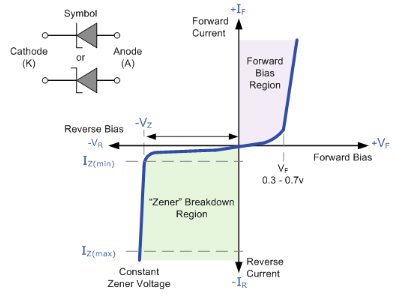
\includegraphics[width=0.7\textwidth]{Images/Zener_IV_Curve.png}
			\caption{Zener diode IV Characteristics}
			\label{fig:zener_iv_curve}
		\end{figure}

		Notice from the figure that at the zener breakdown voltage, the voltage remains basically constant for an increase in the current in the reverse-biased direction.

		This ability of the zener diode to maintain this constant voltage allows it to be used as a voltage regulator, providing a constant output voltage to a load connected in parallel with the zener diode in spite of the voltage ripples in the supply voltage or variations in the load current (so long as this current varies between $I_{Z(min)}$ and $I_{Z(max)}$ as shown in Figure \ref{fig:zener_iv_curve}).

		The voltage the zener is to supply can be determined by resistors connected to the cathode of the zener diode. This resistor must be chosen so as to not exceed the maximum power dissipation of the diode in no-load configuration.

		With the load connected to the zener diode (in parallel), the voltage over the load is exactly that of the zener voltage $V_Z$. The supply voltage $V_S$ must be greater than the zener voltage for the zener to supply this voltage ($V_Z$).

		Another voltage regulator configuration is a circuit that includes a transistor. The zener controlled transistor series voltage regulator will be the circuit of interest in this experiment.

		The zener controlled transistor series voltage regulator circuit consists of an npn transistor and a zener diode with the collector and emitter terminals in series with the load. The reference voltage of the transistor is fed by the zener diode voltage with the transistor acting as a variable resistor based on the base current of the transistor (see the Figure \ref{fig:transistor_zener_circuit} below showing this configuration).

		\begin{figure}[H]
			\centering
			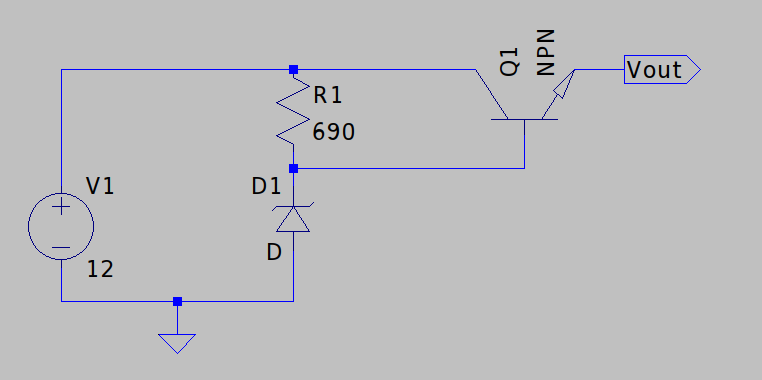
\includegraphics[width=0.7\textwidth]{Images/transistor_zener_circuit.png}
			\caption{Zener controlled transistor series voltage regulator circuit}
			\label{fig:transistor_zener_circuit}
		\end{figure}

		The working principle of the voltage regulator circuit shown in Figure \ref{fig:transistor_zener_circuit} is that a large portion of the change in the supply voltage appears across the transistor while keeping the output voltage constant. The output voltage is given as $V_{out} = V_Z - V_{be}$
	% section theoretical_backgoround (end)

	\section{Equations} % (fold)
	\label{sec:equations}
		Consider for this discussion the figure (Figure ) given below showing the voltage regulator circuit for this experiment.

		\begin{figure}[H]
			\centering
			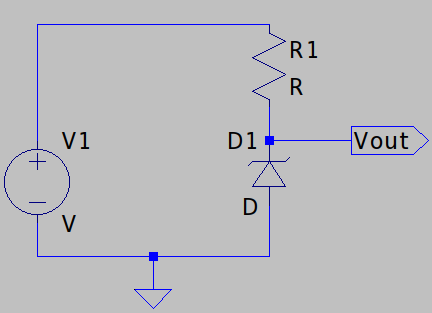
\includegraphics[width=0.7\textwidth]{Images/Regulator_Circuit.png}
			\caption{Zener diode IV Characteristics}
			\label{fig:regulator_circuit}
		\end{figure}

		The zener diode that will be used for this experiment is the 1N4732A. The power that this zener diode must dissipate is $50mW$ and the zener voltage is $4.7V$

		From this the current through the diode with no load connected is calculated below with the max voltage being the supply voltage of $12V$

		\begin{equation}
			\begin{array}{rcl}
				I & = & \frac{P}{V_{max}}\\
				& = & \frac{50\times10^{-3}}{12}\\
				& = & 10.64 \times 10^{-3}A
			\end{array}
		\end{equation}  

		This is the current that should flow through the zener diode. Using this and the zener voltage of $V_Z = 4.7V$, the resistor $R_1$ can be calculated as shown below

		\begin{equation}
			\begin{array}{rcl}
				R_1 & = & \frac{V1 - V_Z}{I}\\
				& = & \frac{7.3}{10.64\times10^{3}}\\
				& = & 686.09 \si{\ohm}
			\end{array}
		\end{equation}  
	% section equations (end)

	\section{Experiment} % (fold)
	\label{sec:experiment}
		From the value calculated for the resistor in the equations section if this report the following circuit was set up as shown below

		\begin{figure}[H]
			\centering
			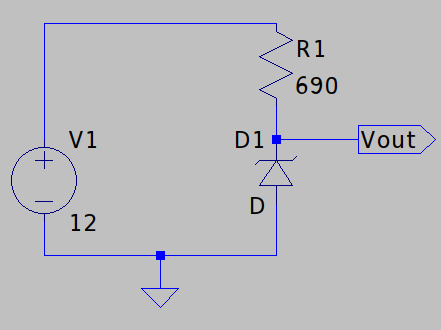
\includegraphics[width=0.7\textwidth]{Images/Part_1_Experiment.png}
			\caption{Zener diode IV Characteristics}
			\label{fig:part_1_experiment}
		\end{figure}

		The voltage we measured at the output terminal was found to be $4.66V$

		By connecting a transistor to the circuit of Figure \ref{fig:part_1_experiment} as show in the figure below 

		\begin{figure}[H]
			\centering
			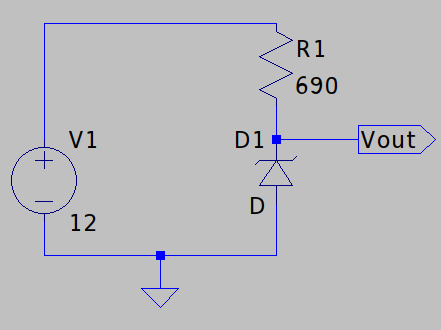
\includegraphics[width=0.7\textwidth]{Images/Part_2_Experiment.png}
			\caption{Zener diode IV Characteristics}
			\label{fig:part_2_experiment}
		\end{figure}

		The output voltage was measured to be $4.25V$. 
	
	% section experiment (end)

	\section{Conclusion} % (fold)
	\label{sec:conclusion}
		With the addition of the transistor, the voltage changed from $4.66V$ to $4.25V$. As discussed in the theoretical background section of this report, the reason for the altered value of $V_{out}$ is explained by the equation given as $V_{out} = V_Z - V_{be}$. $V_{be}$ is the voltage drop inside the transistor due to the resistance of the base-emitter junction.

		The exact zener voltage was not obtained during this experiment (part 1), this is true because the resistor value that was chosen was chosen close to the calculated value of $686.09 \si{\ohm}$ and not the exact value (done so as to make use of resistor values that are supplied in the lab)
	
	% section conclusion (end)

\end{document}